%% This file was auto-generated by IPython.
%% Conversion from the original notebook file:
%% rndsvd.ipynb
%%
\documentclass[11pt,english,fleqn]{article}

%% This is the automatic preamble used by IPython.  Note that it does *not*
%% include a documentclass declaration, that is added at runtime to the overall
%% document.

\usepackage{amsmath}
\usepackage{amssymb}
\usepackage{graphicx}
\usepackage{ucs}
\usepackage[utf8x]{inputenc}

% needed for markdown enumerations to work
\usepackage{enumerate}

% Slightly bigger margins than the latex defaults
\usepackage{geometry}
\geometry{verbose,tmargin=3cm,bmargin=3cm,lmargin=2.5cm,rmargin=2.5cm}

% Define a few colors for use in code, links and cell shading
\usepackage{color}
\definecolor{orange}{cmyk}{0,0.4,0.8,0.2}
\definecolor{darkorange}{rgb}{.71,0.21,0.01}
\definecolor{darkgreen}{rgb}{.12,.54,.11}
\definecolor{myteal}{rgb}{.26, .44, .56}
\definecolor{gray}{gray}{0.45}
\definecolor{lightgray}{gray}{.95}
\definecolor{mediumgray}{gray}{.8}
\definecolor{inputbackground}{rgb}{.95, .95, .85}
\definecolor{outputbackground}{rgb}{.95, .95, .95}
\definecolor{traceback}{rgb}{1, .95, .95}

% Framed environments for code cells (inputs, outputs, errors, ...).  The
% various uses of \unskip (or not) at the end were fine-tuned by hand, so don't
% randomly change them unless you're sure of the effect it will have.
\usepackage{framed}

% remove extraneous vertical space in boxes
\setlength\fboxsep{0pt}

% codecell is the whole input+output set of blocks that a Code cell can
% generate.

% TODO: unfortunately, it seems that using a framed codecell environment breaks
% the ability of the frames inside of it to be broken across pages.  This
% causes at least the problem of having lots of empty space at the bottom of
% pages as new frames are moved to the next page, and if a single frame is too
% long to fit on a page, will completely stop latex from compiling the
% document.  So unless we figure out a solution to this, we'll have to instead
% leave the codecell env. as empty.  I'm keeping the original codecell
% definition here (a thin vertical bar) for reference, in case we find a
% solution to the page break issue.

%% \newenvironment{codecell}{%
%%     \def\FrameCommand{\color{mediumgray} \vrule width 1pt \hspace{5pt}}%
%%    \MakeFramed{\vspace{-0.5em}}}
%%  {\unskip\endMakeFramed}

% For now, make this a no-op...
\newenvironment{codecell}{}

 \newenvironment{codeinput}{%
   \def\FrameCommand{\colorbox{inputbackground}}%
   \MakeFramed{\advance\hsize-\width \FrameRestore}}
 {\unskip\endMakeFramed}

\newenvironment{codeoutput}{%
   \def\FrameCommand{\colorbox{outputbackground}}%
   \vspace{-1.4em}
   \MakeFramed{\advance\hsize-\width \FrameRestore}}
 {\unskip\medskip\endMakeFramed}

\newenvironment{traceback}{%
   \def\FrameCommand{\colorbox{traceback}}%
   \MakeFramed{\advance\hsize-\width \FrameRestore}}
 {\endMakeFramed}

% Use and configure listings package for nicely formatted code
\usepackage{listingsutf8}
\lstset{
  language=python,
  inputencoding=utf8x,
  extendedchars=\true,
  aboveskip=\smallskipamount,
  belowskip=\smallskipamount,
  xleftmargin=2mm,
  breaklines=true,
  basicstyle=\small \ttfamily,
  showstringspaces=false,
  keywordstyle=\color{blue}\bfseries,
  commentstyle=\color{myteal},
  stringstyle=\color{darkgreen},
  identifierstyle=\color{darkorange},
  columns=fullflexible,  % tighter character kerning, like verb
}

% The hyperref package gives us a pdf with properly built
% internal navigation ('pdf bookmarks' for the table of contents,
% internal cross-reference links, web links for URLs, etc.)
\usepackage{hyperref}
\hypersetup{
  breaklinks=true,  % so long urls are correctly broken across lines
  colorlinks=true,
  urlcolor=blue,
  linkcolor=darkorange,
  citecolor=darkgreen,
  }

% hardcode size of all verbatim environments to be a bit smaller
\makeatletter 
\g@addto@macro\@verbatim\small\topsep=0.5em\partopsep=0pt
\makeatother 

% Prevent overflowing lines due to urls and other hard-to-break entities.
\sloppy

\setlength{\mathindent}{0pt}
\setlength{\parindent}{0pt}
\setlength{\parskip}{8pt}
\begin{document}

\section{Rasgele İzdüşümü (Random Projection) ile SVD}

Eger ana matrisimiz $A$'nin cok fazla kolonu var ise bunu bir sekilde
azaltmanin yollarini arayabiliriz. {[}1{]}'e gore bunu yapmanin
yollarindan biri rasgele izdusum hesabidir. Ilk once $n \times k$
boyutunda bir Gaussian rasgele matris $\Omega$ uretiriz. Ardindan
\[ Y = A\Omega \]
hesaplanir. Bu $Y$ uzerinde QR ayristirmasi yapariz, ve elde edilen $Q$
ile
\[ B = Q^T A \]
hesabini yapariz. Ardindan bu matris uzerinde SVD ayristirmasi yapariz,
\[ B = \hat{U}\Sigma V^T \]
ve
\[ U = Q\hat{U} \]
matrisini hesaplariz. Ana fikir suradan geliyor,
\[ A = QQ^TA \]
ki bu standart bir cebir numarasi olurdu, $Q$ yerine rasgele izdusumdan
gelen yaklasiksal $Q$'yu kullanabiliriz, o zaman
\[ A \approx \tilde{Q}\tilde{Q}^TA \]
olacaktir. Yani izdusumden gelen $Q,R$ gercek versiyona yakin. Ustteki
carpimda $R$ yerine $B$ harfi kullaniyoruz, ki $B = \tilde{Q}^T A$
oluyor, yani
\[ A \approx \tilde{Q}B \]
ya da
\[ B \approx \tilde{Q}^T A \].

O zaman Istatistik notlarimiz altindaki \emph{Paralel Matris Carpımı,
Ax, QR ve SVD} yazisinda oldugu gibi $B$'nin SVD'sini alarak yaklasiksal
bir $U$ elde etmek mumkun olacaktir.

Bu yaklasiksal metot isler cunku noktalari yaklasiksal bir altuzaya
yansittiktan sonra elde edilen yeni noktalarin arasindaki mesafelerin
fazla bozulmadan muhafaza edildigi soylenir, daha detayli soylemek
gerekirse, n-boyutlu verileri $O(\log n / \epsilon^2)$ boyutundaki bir
rasgele altuzaya yansitmak, pozitif olasilikla, yeni noktalarin
arasindaki mesafeleri sadece $1 \pm \epsilon$ olcusunde degistirir
{[}2{]}. $Y$'nin, $A$'nin ``menzilini'' iyi temsil ettigi de soylenir.

Test olarak suradaki {[}3{]} veri seti uzerinde gorelim:

\begin{codecell}
\begin{codeinput}
\begin{lstlisting}
import numpy as np
import numpy.random as rand
import numpy.linalg as lin
import matplotlib.pyplot as plt
import pandas as pd

k = 7 # izdusum uzayinin boyutlari
df = pd.read_csv("w1.dat",sep=';',header=None)
A = np.array(df)[:,1:]

print "A",A.shape

rand.seed(1000)

Omega = rand.randn(A.shape[1],k)

Y = np.dot(A, Omega) 

print "Y", Y.shape

Q, R = lin.qr(Y) 

# niye devrigi ile is yaptigimizi altta anlatiyoruz
BT = np.dot(A.T, Q)

print "Q", Q.shape
print "BT", BT.shape

x, x, V = lin.svd(BT)

print 'V', V.shape

Uhat = V.T # cunku B=USV', B'=VSU' U of B icin V' lazim

print "Uhat", Uhat.shape

U = np.dot(Q, Uhat) 

print "U", U.shape

plt.plot(U[:,0],U[:,1],'r+')

plt.hold(True)
        
# compare with real SVD

U, Sigma, V = lin.svd(A);
plt.plot(U[:,0],-U[:,1],'bx')

plt.show()


\end{lstlisting}
\end{codeinput}
\begin{codeoutput}
\begin{verbatim}
A (71, 30)
Y (71, 7)
Q (71, 7)
BT (30, 7)
V (7, 7)
Uhat (7, 7)
U (71, 7)
\end{verbatim}
\begin{center}
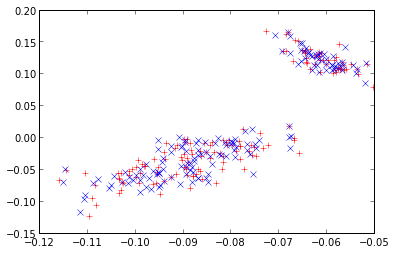
\includegraphics[width=0.7\textwidth]{rndsvd_files/rndsvd_fig_00.png}
\par
\end{center}
\end{codeoutput}
\end{codecell}
Kodlama acisindan, ya da buyuk veri baglaminda baska amaclar icin
{[}4{]} $B = Q^T A$ yerine $B^T = A^T Q$ hesabi yapmak istenilebilir.
Niye? Cunku cikti olarak $n \times k$ matrisi istiyor olabiliriz,
$k \times n$ matrisi istemiyoruz, yani cok olanin satirlar olmasini
istiyoruz, kolonlar olmasini istemiyoruz.

O zaman, elde edilen $B^T$ ise, $B$ uzerinde degil $B^T$ uzerinde SVD
alacagiz demektir, bu da sonuclari birazcik degistirir, yani
\[ B = U\Sigma V^T \]\[ B^T = V\Sigma U^T \]
haline gelir. Yani $B$'nin $U$'sunu elde etmek icin $B^T$'nin SVD'si
sonrasinda ele gecen sonucta $(U_{BT}^T)^T$ yapmak gerekir. Her seyin
hafizada yapildigi durumda bu fark yaratmaz, fakat ``ilerisi icin'',
yani esle / indirge ortamlari icin akilda tutmak faydali olur.

Kaynaklar

{[}1{]} Halko, N., Randomized methods for computing low-rank
approximations of matrices

{[}2{]} Gupta, A., Dasgupta, S., An Elementary Proof of a Theorem of
Johnson and Lindenstrauss

{[}3{]} http://archive.ics.uci.edu/ml/datasets/Breast+Cancer

{[}4{]} http://arxiv.org/abs/1310.4664

\end{document}
